% Compile with XeLaTeX and the supplied APMCM class on TEXINPUTS.
\documentclass{apmcmthesis}
\usepackage{url}
\usepackage[hidelinks,pdfauthor={},pdftitle={Screening Perovskites When All Exact Targets Are Hidden}]{hyperref}
\tihao{D}
\baominghao{}
\newcommand{\FoldRows}{All & Direct & 27/83 & 11.256 & 0.080--12.475 \\
All & Mixture & 38/83 & 12.475 & 0.089--13.521 \\
Q2 & Direct & 10/10 & 11.252 & 10.106--12.116 \\
Q2 & Mixture & 10/10 & 8.009 & 0.675--12.116 \\
Q3 & Direct & 14/50 & 11.569 & 1.118--43.556 \\
Q3 & Mixture & 23/50 & 13.521 & 4.850--19.594 \\}
\newcommand{\DescOne}{0.0376}
\newcommand{\FitOne}{100.6621}
\newcommand{\ScoreOne}{0.0352}
\newcommand{\DescFull}{0.0227}
\newcommand{\FitFull}{103.3896}
\newcommand{\ScoreFull}{0.0819}
\newcommand{\PoolTwo}{0.0234}
\newcommand{\EncodeTwo}{0.0231}
\newcommand{\SolveTwo}{0.7431}
\newcommand{\CheckTwo}{0.0802}
\newcommand{\ScanTwo}{1.2000}
\newcommand{\TiedTwo}{71}
\newcommand{\FinalistsTwo}{288}
\newcommand{\CoeffLowTwo}{-122}
\newcommand{\CoeffHighTwo}{0}
\newcommand{\PoolThree}{0.0109}
\newcommand{\EncodeThree}{0.0233}
\newcommand{\SolveThree}{0.7431}
\newcommand{\CheckThree}{0.0808}
\newcommand{\ScanThree}{2.5000}
\newcommand{\TiedThree}{70}
\newcommand{\FinalistsThree}{286}
\newcommand{\CoeffLowThree}{-123}
\newcommand{\CoeffHighThree}{0}

\renewcommand{\baselinestretch}{1.10}
\setlength{\parindent}{0pt}
\setlength{\parskip}{.45em}
\setlength{\headheight}{15pt}
\setcounter{tocdepth}{1}
\setlength{\emergencystretch}{1.2em}
\captionsetup{font=small,labelfont=bf,justification=raggedright,singlelinecheck=false}
\newcommand{\Vh}{\widehat V}
\newcommand{\noo}{\mathrm{NO}_2}
\newcommand{\ooo}{\mathrm O_3}
\newcommand{\foo}{\mathrm{FO}_2}
\newcommand{\subhead}[1]{\par\smallskip{\large\bfseries #1}\par\nopagebreak}
\begin{document}
\pagestyle{mainmatterstyle}
\begin{abstract}
\begin{center}
{\Large\bfseries Screening Perovskites When All Exact Targets Are Hidden}\\[3pt]
{\large A band-gap surrogate and an audited 8-bit QUBO search}
\end{center}
All 19 zero-violation compositions in the 18,928-candidate grid belong to the hidden set. The public records nevertheless contain a measurable signal for screening. Every labeled zero-gap material has coincident band edges. Under the contest loss this implies a violation of at least 10.8658. We use a composition-based classifier to estimate the probability of a positive gap and fit separate violation regressions for the two regimes.

On 3,969 validation compositions from unseen element pairs, the resulting model retrieves 13 of the 27 materials with $V<1$ in its first 50 choices, compared with six for direct regression. A second training seed gives 15 versus ten. The improvement has a limit at a budget of one. On the three-family validation pool, the first choice has observed $V=11.4923$ at the primary seed, although the attainable minimum is 0.0400.

After refitting on all public labels, the full-pool surrogate selects $\mathrm{LaTiO_2N}$ for fixed $\noo$ ($\Vh=6.924382$) and $\mathrm{SnTiO_3}$ for the three-family problem ($\Vh=3.268113$). The first material has a hidden label. The second has public training $V=0.001419$. Restricting the three-family search to unseen pairs selects $\mathrm{LaTiO_2N}$ again.

Direct 8-bit conversion changes the best legal pair in all six whole-grid settings tested on the three-family score table. We partition the table into $4\times4$ blocks, encode bounded integer costs, solve each block with the Kaiwu SDK on a CPU, and resolve ties using the original predictions. All 338 block solves pass exhaustive feasibility and energy checks. Both final selections match exact enumeration. At this scale a direct array scan is cheaper. The larger uncertainty is the physical loss at a previously unseen composition.
\keywords{perovskite screening, grouped validation, band-gap mixture, QUBO, coefficient precision}
\end{abstract}
\clearpage
\tableofcontents
\clearpage
\section{Problem formulation and data}
Castelli et al.\ screened cubic perovskites for light-driven water splitting \cite{castelli}. A composition with a suitable gap can still fail on band alignment or stability. Problem D combines these failures into one score and asks for a single composition in each of two search spaces \cite{contest}. The public records contain no zero-loss composition, making screening of unseen candidates the central challenge.

\subhead{Problem restatement}
Q1 requires one predicted violation per hidden composition. Q2 selects one material in the fixed $\noo$ family. Q3 selects one material across $\ooo$, $\noo$ and $\foo$. The contest supplies the energy thresholds and eligible pools; the violations of hidden candidates and the selected compositions are the outputs.

For ordered sites $A$ and $B$ and anion family $X$, denote formation energy, GLLB-SC gap, valence edge and conduction edge by $e,g,v,c$, respectively, in eV. GLLB-SC is a computational approach to estimating band gaps \cite{kuisma}. We retain the edge convention in the supplied data. The five penalties represent excessive formation energy, a gap below or above its window, and a violation of either band-edge threshold. With $[t]_+=\max(0,t)$ and all energy scales in eV, the dimensionless contest loss is
\begin{align}
 d&=(e-0.21,\;1.4-g,\;g-3.1,\;5.73-v,\;c-4.50),\notag\\
 V(A,B,X)&=\sum_{j=1}^5 [d_j/0.5]_+^2. \label{eq:loss}
\end{align}
Equation~\eqref{eq:loss} includes equality in its zero set. The organizers report 19 compositions with $V=0$ and 15 under the strict physical inequalities. We use the former convention. Recomputing $V$ from the four rounded public quantities gives a maximum absolute discrepancy of $1.02\times10^{-5}$. We fit the supplied six-decimal target after this check.

The partitions in Table~\ref{tab:data} keep all seven anion families of each ordered pair together.

\begin{table}[htbp]
\caption{Official partitions. Each pair contributes seven families to its partition. The hidden exact-target count comes from the organizers.}\label{tab:data}
\centering\begin{tabular}{lrrrr}
\toprule Partition & Pairs & Rows & $V=0$ & $V<1$ observed\\\midrule
Training (02) & 1,608 & 11,256 & 0 & 83\\
Selection (03) & 567 & 3,969 & 0 & 27\\
Holdout (04) & 529 & 3,703 & 19 & unavailable\\\bottomrule
\end{tabular}
\end{table}

The grid contains $52^2\times7$ compositions, including $A=B$. The pair sets are disjoint. The seven families are O3, NO2, FO2, N2O, N3, O2S and FNO. File 06 repeats public compositions without labels. We use 02 for Q1 training, 03 for model selection and 04 for predictions. Q2 and Q3 use a separate fit on 02 and 03. The problem permits pools 07 or 11 for Q2 and 08 or 12 for Q3. We use blind pools 11 and 12 for the final prospective selections and retain full pools 07 and 08 as optimization benchmarks. Sorting by identifier breaks exact score ties.

\subhead{Solution route and modeling assumptions}
For Q1, we learn from labeled compositions and validate on unseen ordered pairs because hidden candidates lack physical properties. For Q2 and Q3, we refit on the public labels and freeze the predicted scores. We minimize over Q3 families within each pair and compare the decoded 8-bit solution with a direct scan to check whether encoding preserves the score minimum.

The ideal cubic prototype is given. We use ordered composition and element descriptors at inference, so the model cannot distinguish different structures with the same composition and does not use measured geometry or density functional theory (DFT) outcomes as predictors. The empirical convention that zero-gap records have coincident band edges is the condition for the metallic lower bound below.

Figure~\ref{fig:workflow} shows where the use of file 03 changes. Its labels first evaluate candidate predictors. Once the model design is fixed, those labels join the training data for the two selection tasks.
\begin{figure}[htbp]
\centering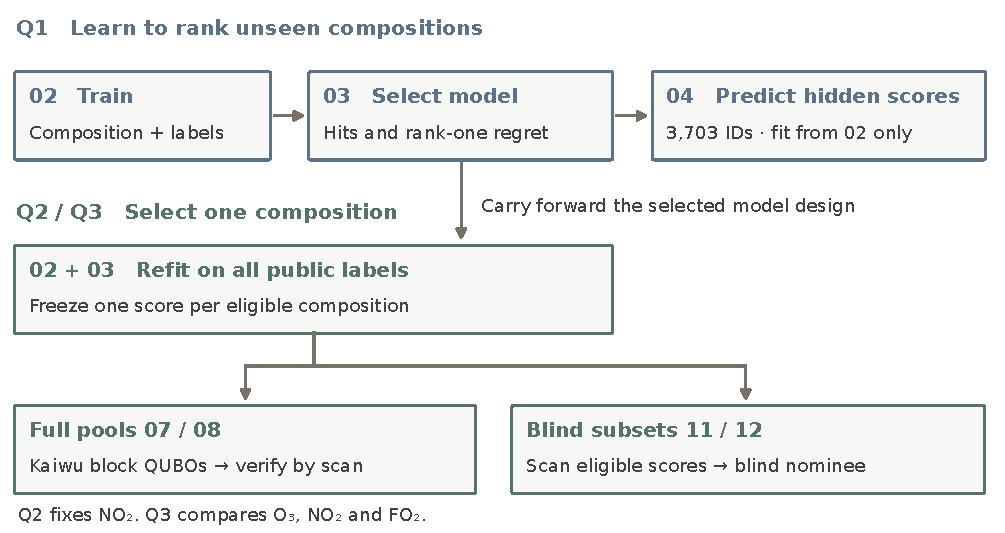
\includegraphics[width=\linewidth]{figures/workflow.pdf}
\caption{Data flow across the three tasks. Q1 checks ranking against observed violations. Q2 and Q3 check the decoded minimum against the frozen score table. The figure shows the historical mixture benchmark. Final blind selections additionally use the membership-constrained solves described in Model III.}\label{fig:workflow}
\end{figure}

\subsection{Model assumptions and notation}
\begin{enumerate}
\item Candidate compositions follow the supplied cubic prototype. A and B are ordered sites; equal elements are allowed.
\item Inference uses composition and deterministic element descriptors only. Measured physical properties are training labels, not hidden-set inputs.
\item The empirical zero-gap convention $v=c$ is retained for the metallic lower bound.
\item Public validation near-targets provide a development proxy; their distribution need not match hidden exact targets.
\end{enumerate}
\begin{table}[htbp]\centering\small\caption{Principal notation.}\begin{tabular}{ll}\toprule Symbol & Meaning\\\midrule
$A,B,X$ & Ordered metal sites and anion family\\
$e,g,v,c$ & Formation energy, gap and two band edges (eV)\\
$V,\widehat V$ & Observed loss and uncalibrated predicted score\\
$p,L$ & Positive-gap probability and metallic loss bound\\
$C,q,P$ & Raw cost table, integer costs and constraint penalty\\
$H_k,R_1$ & Near-target hits in $k$ checks and rank-one excess loss\\\bottomrule\end{tabular}\end{table}

\subsection{Why A and B must remain ordered}
The contest supplies an ideal cubic prototype. To isolate the effect of site assignment in the illustration, we hold its fractional coordinates fixed and place A at the corners, B at the body center and the anions at the face centers \cite{aflow}. The eight corners contribute $8/8=1$ A atom per cell. The six faces contribute $6/2=3$ anions. B has six nearest anion neighbors in the illustrated octahedron, while the periodically repeated face centers give A twelve nearest anion neighbors. The contest family label specifies the composition of the three anions. For example, NO2 supplies one N and two O per formula unit. For the blind candidate this fixes stoichiometry only; the data leave the O/N site ordering unresolved.

Figure~\ref{fig:cell} compares two DFT records at reversed site assignments. The exchange arrow connects two separately calculated compositions.

\begin{figure}[htbp]
\centering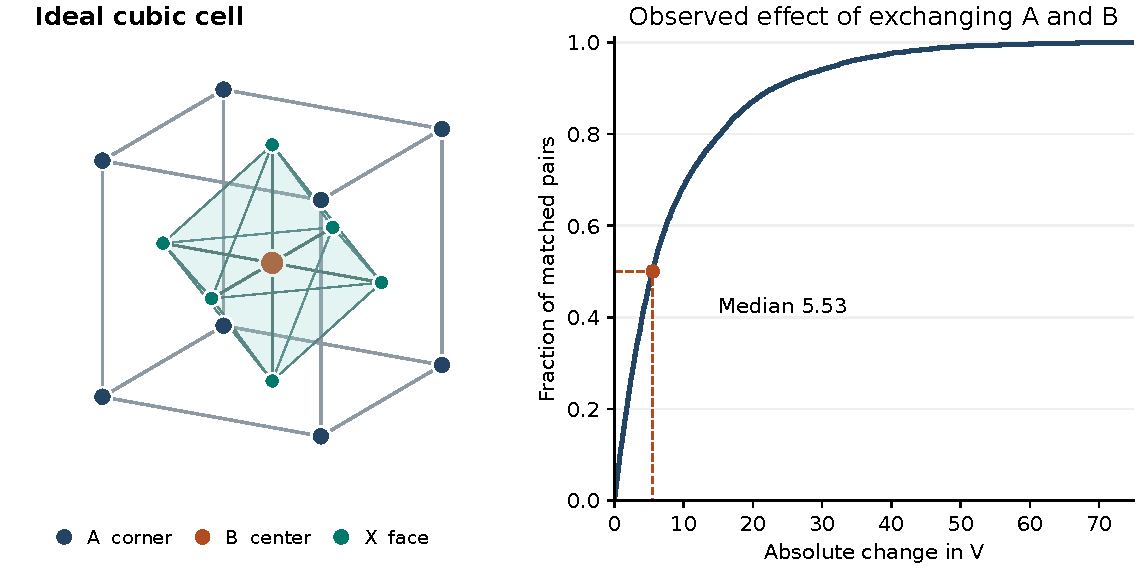
\includegraphics[width=.98\linewidth]{figures/crystal_sites.pdf}
\caption{Exchanging the corner and central cations in the ideal cubic prototype \cite{aflow}. Gap and violation are the public DFT values for each composition.}\label{fig:cell}
\end{figure}

We matched each public record $(a,b,x)$ with $(b,a,x)$ when both were labeled, excluded $a=b$, and counted each reciprocal pair once. Among 5,971 matches, the median absolute difference is 5.5296, with quartiles 2.2672 and 12.6046. A predictor that gives both records the same output $h$ incurs
\[
 \tfrac12\{|V(a,b,x)-h|+|V(b,a,x)-h|\}\ \geq\
 \tfrac12 |V(a,b,x)-V(b,a,x)|.
\]
Averaging the right-hand side gives an unavoidable MAE of at least 4.6805 on these 11,942 matched rows for a site-invariant predictor. This bound concerns the matched sample and must be compared on that same sample. It motivates retaining separate A and B descriptors before fitting.

The Sn--Ti pair illustrates the size of this effect. Public $\mathrm{SnTiO_3}$ has $g=2.50$ eV and $V=0.001419$. Its reversed assignment $\mathrm{TiSnO_3}$ has $g=0$ and $V=18.422244$. For $\mathrm{SnTiO_3}$ the supplied cubic lattice parameter is 3.969143~\AA. Lattice parameters and volumes are available only in labeled records and do not enter the score of a new composition.

\section{Model I: Composition-based surrogate}
Of 15,225 public rows, 14,652 have $g=0$. Each of these records has $v=c$. We use this empirical band-edge convention when modeling a zero-gap candidate; applying the bound to another dataset requires checking the convention there. Set both edges to $t$. The gap alone contributes $(1.4/0.5)^2=7.84$. Between 4.50 and 5.73, the two edge penalties form a convex quadratic symmetric about $t=5.115$. Outside that interval their sum increases. Formation energy can only add a nonnegative penalty. Hence under the observed coincident-edge convention
\begin{equation}
 V_{\rm metal}\ \geq\ L=7.84+
 \frac{(5.73-4.50)^2}{2(0.5)^2}=10.8658. \label{eq:metal}
\end{equation}
The smallest metallic values observed against the bound in Eq.~\eqref{eq:metal} are 10.865834 in training and 10.866614 in validation. A zero-gap record thus teaches the model where a near-target is physically unlikely. At prediction time the gap is unknown.

\clearpage
\subsection{Which physical failures dominate the screen?}
The metallic lower bound resolves the gap and both edge penalties jointly. For a metal with common edge $t$, the vertical distance above the following curve is exactly the formation-energy penalty, up to the supplied rounding:
\[
 B(t)=7.84+[ (5.73-t)/0.5 ]_+^2+[(t-4.50)/0.5]_+^2 .
\]
Moving the common edge to the left alleviates the CBM violation while increasing the VBM violation. Moving it to the right has the opposite effect. Their thresholds are separated by 1.23 eV. Figure~\ref{fig:regimes} shows why neither edge adjustment can compensate for zero gap.

\begin{figure}[ht]
\centering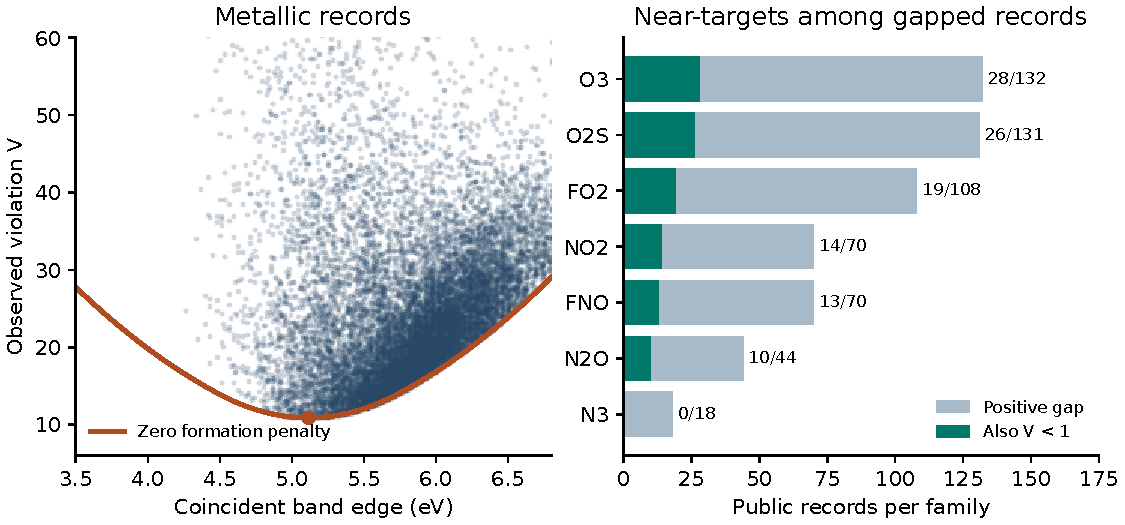
\includegraphics[width=\linewidth]{figures/physical_regimes.pdf}
\caption{Left, labeled metallic records from files 02 and 03 in the displayed edge and violation window. The curve gives $B(t)$ and the dot its minimum. Right, each family has 2,175 labeled records. Numerators count $V<1$ records and denominators count positive-gap records.}\label{fig:regimes}
\end{figure}

Positive gap narrows the public screen from 15,225 records to 573 and retains all 110 with $V<1$. Even with the true gap known, only $110/573=19.2\%$ of the gapped records pass this relaxed test. In O3, 28 of 132 gapped compositions have $V<1$. In NO2, the ratio is 14 of 70, and in N3 none of 18 passes. These counts are descriptive. In particular, the hidden set was constructed to contain the exact targets, which changes the interpretation of any full-population prevalence estimate.

At inference the gate supplies only an estimated probability. In Eq.~\eqref{eq:mix}, an increase $\delta$ in the predicted metallic probability increases the predicted score by $\delta(f_0^\prime-f_+^\prime)$ with the clipped branch estimates held fixed. The effect is greatest when the two branches disagree. This is why a confidently wrong metallic assignment can hide a promising material. Conversely, a candidate assigned high positive-gap probability still has to survive its branch's estimated formation and edge penalties. The validation experiment below tests the combined effect in the order in which materials would be checked.



\subhead{A surrogate with observable training labels}
Composition-based descriptors have proved useful in inorganic property prediction \cite{ward}. For each metal site separately we use atomic number, Pauling electronegativity, periodic-table row and group from pymatgen \cite{ong}. Three categorical fields $A,B,X$ bring the total to eleven. This preserves site order and assumes the supplied cubic prototype throughout.

CatBoost handles the categorical inputs \cite{catboost}. Let $p(z)$ estimate $\Pr(g>0\mid z)$ from composition features $z$. Let $f_+(z)$ and $f_0(z)$ be the violation estimates from regressors trained on positive-gap and zero-gap records, respectively. If the gate were the true regime probability and the branches the corresponding conditional means, the law of total expectation would give the conditional mean violation. Our fitted and clipped components approximate that construction; their weighted sum is a screening score, rather than a calibrated probability of satisfying all constraints. This motivates
\begin{equation}
 \Vh(z)=p(z)\max(0,f_+(z)) + (1-p(z))\max(L,f_0(z)).
 \label{eq:mix}
\end{equation}
File 02 supplies 432 positive-gap and 10,824 metallic outcomes for fitting the gate. This classification label is observed even though the exact screening target never occurs in 02. Soft weighting keeps every candidate eligible. A composition receiving a high $p$ may still fail the band-edge or formation-energy requirements.

We compare with one direct regressor for $V$ using identical descriptors, 350 boosting iterations per component, depth 5, learning rate 0.08, four CPU threads and seeds 26 and 42. The mixture fits three components. Holding depth and descriptors fixed, we also fit direct regressors with 700 and 1,050 trees. The first budget matches the nominal training-row passes of the gate plus its two disjoint branches, and the second matches their total tree count. We carry seed 26 forward to use one fixed score table for both optimization problems. File 03 was reused for exploratory model selection. Its metrics describe development performance. The same model-selection reuse also limits interpretation of the later grouped and stress diagnostics: they assess the chosen design, rather than a fully nested selection procedure. The Q1 deliverable, \texttt{q1\_holdout.csv}, contains one composition-only prediction for each of the 3,703 hidden IDs.

\clearpage
\subsection{Following one composition through the predictor}
Consider $\mathrm{InTiO_3}$, the first-ranked seed-26 mixture candidate in the Q3 validation subset. Its actual zero gap is available only when we evaluate the prediction. During screening, the classifier puts probability 0.5426 on a positive gap. The two regressors then disagree by 9.3786 score units. Figure~\ref{fig:gate} shows the site identities that enter the predictor. The shared oxygen connects two B-centered octahedra. This ideal repeat illustrates the composition; the fitted gate uses the eleven site descriptors described above.

\begin{figure}[ht]
\centering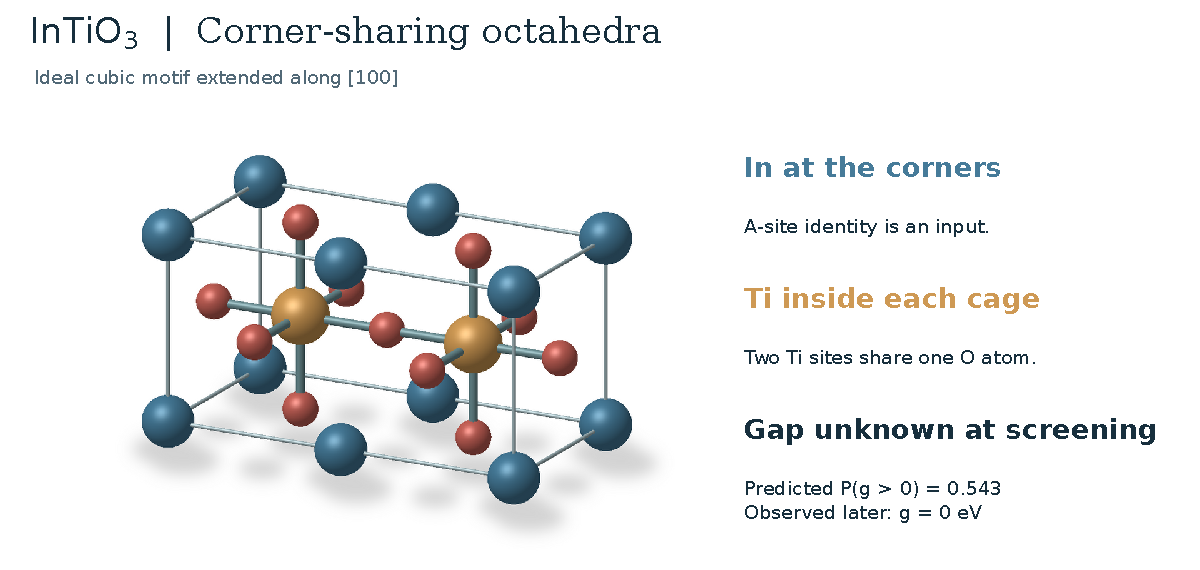
\includegraphics[width=\linewidth]{figures/gate_mechanism.pdf}
\caption{Two ideal cubic repeats for validation ID 16911. In occupies the blue corner sites, Ti the gold centers, and O the red face sites. The positive-gap probability was estimated from composition before the observed metallic label was consulted.}\label{fig:gate}
\end{figure}

Writing $m$ and $u$ for the clipped metallic and positive-gap scores, respectively, gives $\Vh=m-p(m-u)$. The metallic branch contributes approximately $0.4574(11.9231)=5.45$ and the positive-gap branch $0.5426(2.5444)=1.38$. The arithmetic explains two features of this selection. First, a hard decision at $p=0.5$ would report only 2.5444, discarding a material portion of the expected violation. Second, a 0.10 increase in the positive-gap probability would lower the score by 0.938 with both branch estimates fixed. That sensitivity is large enough to matter among closely ranked candidates.

The gate also imposes a one-sided condition on very low scores. Since $u\geq0$ and $m\geq L$, Eq.~\eqref{eq:mix} gives
\[
 \Vh\geq (1-p)L,\qquad
 \Vh<1\ \Longrightarrow\ p>1-1/L\simeq0.9080 .
\]
This is a necessary condition on a \emph{predicted} score below one. A physically good but uncertain material may still receive a much larger score. Ranking by the continuous mixture keeps that material available when no candidate crosses a fixed prediction threshold. Conversely, assigning probability greater than 0.908 does not guarantee good band alignment or formation energy.

\clearpage
\subsection{A controlled test of the probability gate}
To isolate the effect of gating, we hold the learned branch functions $u$ and $m$, the seed, descriptors and train--validation split fixed. Only the mixing weight changes. The constant rule assigns the file-02 positive-gap fraction $432/11256$ to every composition. The hard rule replaces the predicted probability by $\mathbf{1}[p\geq0.5]$. The soft rule uses $p$ itself. A fourth, diagnostic rule routes each validation record by its observed gap label, an input unavailable on the blind pool. Replaying the soft rule reproduces all 3,969 archived validation scores within $10^{-8}$.

\begin{table}[ht]
\caption{Changing only the gate on file 03. Hits count $V<1$ among the first 50. All-family and Q3 denominators are 27 and 11 available near-targets. The final column gives observed $V$ at Q3 rank one.}\label{tab:gate}
\centering\small\begin{tabular}{lrrrr}
\toprule Routing weight & All-family MAE & All hits & Q3 hits & Q3 first $V$\\\midrule
Training prevalence & 2.942 & 4 & 2 & 10.895\\
Hard decision & 2.909 & 8 & 1 & 11.492\\
Soft probability & 2.949 & 13 & 5 & 11.492\\
Observed gap (diagnostic) & 2.678 & 20 & 9 & 1.488\\\bottomrule
\end{tabular}
\end{table}

The hard decision gives a slightly smaller mean error than the soft mixture, yet it retrieves five fewer near-targets at budget 50 across all families. Many promising compositions fall below the hard threshold. Of the 141 validation materials with a positive gap, the classifier flags only 14 at $p\geq0.5$, alongside four false positives. Its precision there is $14/18$, while its recall is $14/141$. A hard rule makes the 127 missed positive-gap records share the metallic scoring regime with most of the validation set.

As a probability score for the positive-gap event, the gate attains a Brier score of 0.0273, compared with 0.0343 for the constant training prevalence. Average precision is 0.367 against a validation event frequency of 0.0355. These metrics concern metallicity; the exact contest target never occurs in the public labels. On Q3, even access to the observed regime yields a first choice with $V=1.4884$, above the near-target threshold. Improving the gate alone would still leave the regression problem of ranking positive-gap materials by their joint physical penalties.


\section{Model evaluation and sensitivity}
For an ordered shortlist $S_k$ define $H_k=\sum_{i\in S_k}\mathbf1[V_i<1]$. Recall divides $H_k$ by the number of such targets in the relevant pool. For a one-choice decision $i^*$, labeled-pool regret is $R_1=V_{i^*}-\min_i V_i$. The expected number of $V<1$ hits in 50 random draws without replacement from the entire validation pool is $50(27/3969)=0.34$. Table~\ref{tab:val} compares this screening budget with the first-choice outcomes.

\begin{table}[htbp]
\caption{Performance on 567 unseen ordered pairs. Mean absolute error (MAE), root mean squared error (RMSE) and hits use all 3,969 rows. The last columns give observed $V$ at rank one in each restricted pool. Decimal columns show three places.}\label{tab:val}
\centering\small\begin{tabular}{lrrrrrrr}
\toprule Fit & Seed & \multicolumn{1}{c}{MAE} & \multicolumn{1}{c}{RMSE} & $H_{20}$ & $H_{50}$ & \multicolumn{1}{c}{Q2 first} & \multicolumn{1}{c}{Q3 first}\\\midrule
Direct &26&3.016&5.000&2&6&8.562&11.492\\
Mixture &26&2.949&4.828&8&13&10.927&11.492\\
Direct &42&3.013&4.945&3&10&11.540&46.240\\
Mixture &42&3.025&4.902&9&15&11.084&12.670\\\bottomrule
\end{tabular}
\end{table}

The mixture retrieves 48.1\% and 55.6\% of the 27 near-targets at $k=50$ for seeds 26 and 42. In Q2 it retrieves all four validation near-targets in 50 checks under both seeds, yet its first choice has $V>10$. In Q3, the seed-26 mixture and direct fits retrieve five and one of eleven near-targets. Both select $\mathrm{InTiO_3}$ first, with regret $11.49225-0.04000=11.45225$ (Figure~\ref{fig:screen}). Increasing the direct-model tree count to 700 and 1,050 raises its Q3 hit count from one to two and four at seed 26, with the same first choice. At seed 42 the counts are three, five and five, against six for the mixture. The shortlist advantage narrows as the direct model grows. The appendix subsection on screening curves gives the full curves for both seeds.

\begin{figure}[htbp]
\centering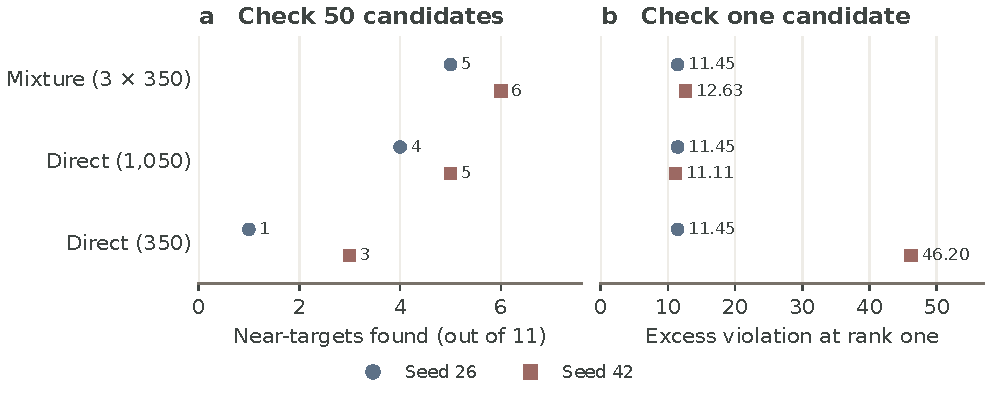
\includegraphics[width=.97\linewidth]{figures/q3_budget.pdf}
\caption{Two decisions on the same 1,701 Q3 validation compositions. At 50 checks the mixture finds one more of the eleven near-targets ($V<1$) than the 1,050-tree direct fit under each seed. At one check, smaller excess violation is better. All three fits choose the same material at seed 26; at seed 42 the larger direct fit has the lowest excess.}\label{fig:screen}
\end{figure}

\clearpage
\subsection{How much of the shortlist survives a change of sample or seed?}
The validation sample contains 567 ordered metal pairs. Each pair contributes seven associated families, and we use the pair as the resampling unit. To assess sensitivity to the mix of pairs, we draw 567 pairs with replacement, retaining the whole family group and its multiplicity. On each resample we rank the records using the already fitted seed-26 predictors and count $V<1$ hits among the first 50. We use the same draw for both methods. This paired design preserves the dependence of their predictions on the same materials.

\begin{figure}[ht]
\centering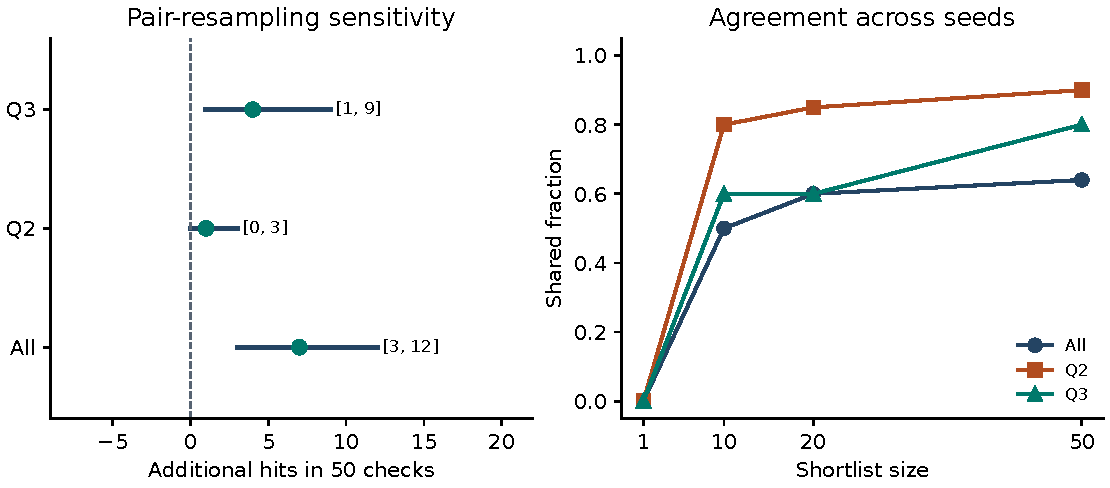
\includegraphics[width=\linewidth]{figures/validation_stability.pdf}
\caption{Left, observed mixture-minus-direct hit counts at budget 50 (dots) and the 2.5th to 97.5th percentiles over 2,000 resampled pair sets (segments). Right, the fraction of each mixture shortlist shared by training seeds 26 and 42 on the original validation set.}\label{fig:stability}
\end{figure}

Across all families the observed improvement is seven hits, with a resampling range of three to twelve (Figure~\ref{fig:stability}). For Q2 the improvement is one and the interval reaches zero. Only four near-targets are present in that validation pool, leaving little room for a large observed gain. For Q3 the gain is four with a range of one to nine. The intervals describe sensitivity conditional on the trained models and the empirical pair distribution. Resampled duplicates count toward both hit totals and the 50-record budget. These are diagnostics of the metric, rather than prospective yields for 50 distinct new experiments.

We separately intersect the predicted shortlists from seeds 26 and 42. At $k=50$, 45 of 50 Q2 candidates and 40 of 50 Q3 candidates are shared. At $k=1$ the two seeds select different IDs in both pools. We therefore report the first choice on the frozen score table together with its validation regret. Seed agreement at a larger budget supports a follow-up shortlist but supplies little assurance about which single material a laboratory should measure first.


\section{Robustness tests and task-specific model choice}
We repeat the comparison inside file 02 with five shuffled folds of complete $(A,B)$ pairs. Each model uses four folds for fitting and ranks the fifth. Spending 50 checks in each held-out pool gives 250 checks per row of Table~\ref{tab:fold}. The five regrets describe variability across held-out compositions. The folds overlap in training data.
\begin{table}[htbp]
\caption{Five grouped folds within 02. The denominator counts all observed $V<1$ targets across the five held-out pools.}\label{tab:fold}
\centering\small\begin{tabular}{llrrr}
\toprule Pool & Method & Hits / targets & Median $R_1$ & Range of $R_1$\\\midrule
\FoldRows
\bottomrule\end{tabular}
\end{table}
In Q3 the mixture finds more near-targets over the five shortlists, yet its median first-choice regret is larger. A second stress test removes every pair containing $V<0.25$ from the training portion of file 02 and adds background pairs to form a 322-pair holdout. All 29 such targets lie among 2,254 held-out records. Across two background selections, direct regression retrieves five of 29 in its top 50 and the mixture retrieves nine. On the three-family subset the counts are five and seven of 20. Between the two background-pair samples, mixture rank-one $V$ changes from 13.8461 to 0.4756 while the attainable minimum is 0.0004 in both. These runs share the same targets. Their prevalence is 1.29\%, compared with 0.10\% for exact zeros on the contest grid.

\subhead{When predicting each physical quantity helps}
Public solution notes discussed property-first prediction and retaining zero-gap records \cite{note1,note2}; the implementations and numerical comparisons reported here are our experiments. These references acknowledge that influence rather than claim originality for those general suggestions. In our property-first comparison, four 220-tree regressors separately predict $e,g,v,c$ before applying Eq.~\eqref{eq:loss}. The mixture uses the classifier and conditional regressors in Eq.~\eqref{eq:mix}. At seeds 26 and 42, the property model selects a Q2 composition with observed $V=0.36$, versus 10.93 and 11.54 for a 220-tree direct fit. In Q3 both property fits choose $\mathrm{CaZrO_3}$ with $V=46.24$. At seed 26 its predicted gap is 2.19 eV, inside the window. The observed gap is 6.50 eV. The upper-gap term alone is $((6.50-3.10)/0.50)^2=46.24$. Average property accuracy conceals this error at the selected extreme. We retain the mixture for Q1 and the Q3 screening analysis. For the final Q2 single-choice task, we choose the property-first model using its better observed first-choice performance under both seeds. For a single Q2 choice, the property-first fit also improves on the mixture (observed $V=10.927$ and $11.084$ for the two mixture seeds). We revisit this choice on the blind Q2 pool after refitting both models. The task-specific choice uses development evidence, so its hidden-set performance still requires independent verification.

\subhead{Rank-ensemble sensitivity}
We additionally average the ascending within-pool ranks of direct, mixture and property-first predictions with equal weights. Q2 rank-one observed losses are 10.927 and 11.981 at seeds 26 and 42, versus 0.360 for property-first under both seeds. Q3 ensemble losses are 3.240 and 21.160, versus 11.492 and 12.670 for the mixture. The inconsistent change across Q3 seeds supplies no stable reason to switch to this ensemble. Full results are in \texttt{rank\_ensemble.csv}.
\clearpage
\subsection{Reading a near miss and a false positive from their band edges}
The band-edge thresholds and the gap window test different aspects of a prediction. Figure~\ref{fig:bands} uses the contest's edge convention, plotting larger reported edge values lower on the page. Each horizontal solid level is a CBM or VBM value; its height can be compared across all three columns. The dotted levels show the two contest cutoffs. For a successful candidate, the CBM should lie above its line in the drawing and the VBM below its own line.

\begin{figure}[ht]
\centering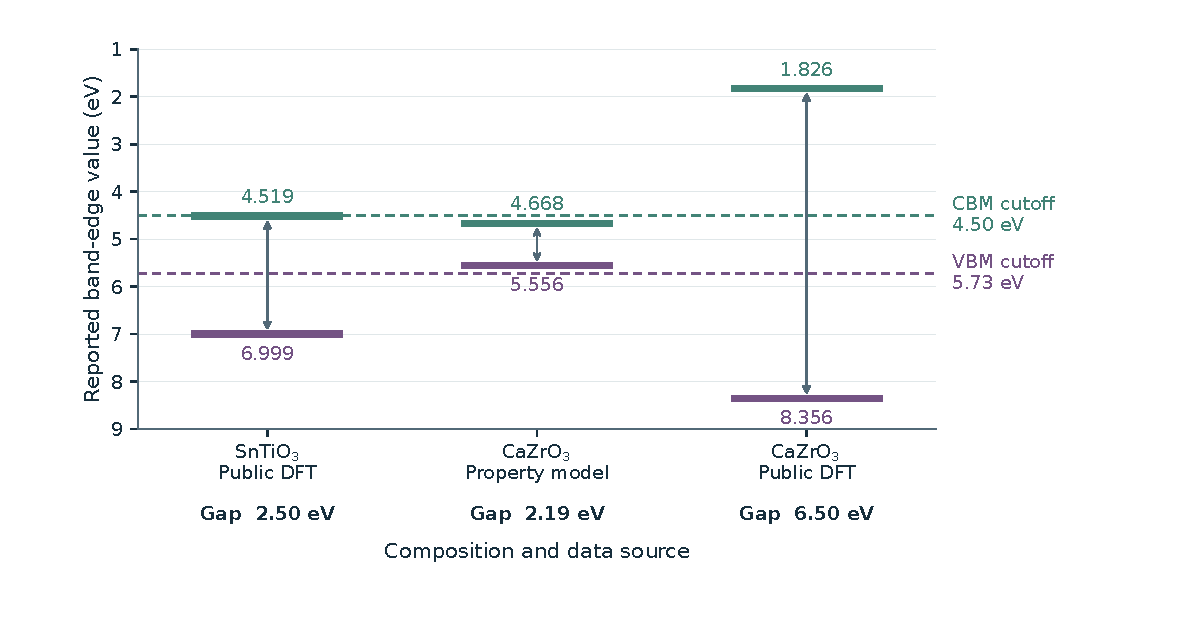
\includegraphics[width=\linewidth]{figures/band_edges.pdf}
\caption{Band-edge levels in eV for the public Q3 winner and the Q3 failure of the seed-26 property model. Arrows span the two edge estimates. Below each column is the separately reported or predicted GLLB-SC gap field used in the objective. Energies follow the file's reference convention.}\label{fig:bands}
\end{figure}

For $\mathrm{SnTiO_3}$, the CBM lies 0.018833 eV beyond its cutoff, a difference too small to resolve easily at the figure scale. For $\mathrm{CaZrO_3}$ the observed edges both pass, but the observed gap is 6.50 eV. It exceeds the upper limit by 3.40 eV and produces the entire observed violation of 46.24.

The middle column explains how the four-property model can rank that material first. It predicts $g=2.1883$ eV, with both small band-edge violations and a passing formation energy, for a total predicted $V=0.2342$. Its independently fitted edges imply $5.5559-4.6680=0.8879$ eV, far from its own gap estimate. In the public DFT record the analogous difference is 6.53 eV, close to the tabulated 6.50 eV. The discrepancy between the model's two estimates of the gap provides a composition-level warning that could be checked before spending a single assay. The following sensitivity test evaluates this warning across all Q3 validation pairs.

\clearpage
\subsection{Can a consistency check rescue a one-choice screen?}
The $\mathrm{CaZrO_3}$ failure suggests a testable diagnostic. Define
\[
 D(z)=\big|\hat g(z)-(\hat v(z)-\hat c(z))\big|.
\]
All three terms are predictions from the property-first model, so the diagnostic could be computed before measuring a candidate. It checks whether the two representations of the gap agree. A small residual can also occur when both representations are wrong in the same direction.

\begin{figure}[ht]
\centering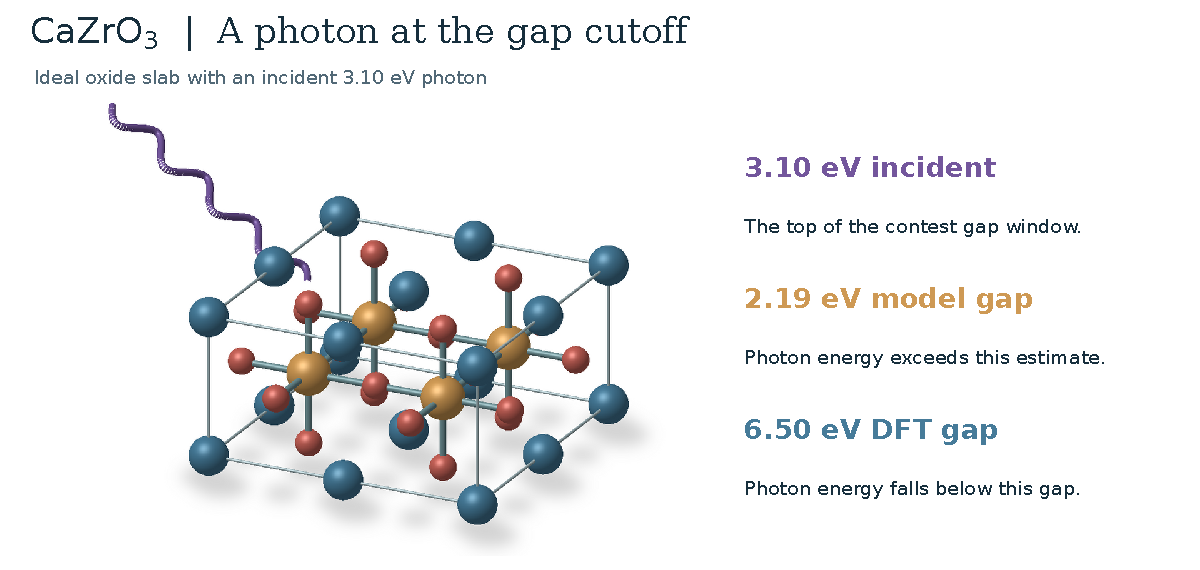
\includegraphics[width=.95\linewidth]{figures/property_tests.pdf}
\caption{An incident photon at the 3.10 eV screening cutoff approaches an ideal fragment of $\mathrm{CaZrO_3}$. The wave is symbolic. Its energy exceeds the model gap but falls below the public DFT gap. This compares energy thresholds only; the files supply no absorption spectrum for this illustration.}\label{fig:physicaltests}
\end{figure}

At 3.10 eV, a photon carries about the energy of 400 nm light ($\lambda=hc/E$). Figure~\ref{fig:physicaltests} uses it to expose the practical consequence of the gap discrepancy. Whether a transition actually absorbs light also depends on selection rules and the optical response.

We test a veto on the 1,701 Q3 validation records: discard predictions with $D>\tau$ and select the remaining candidate with the smallest property-first violation. Table~\ref{tab:veto} reports both seeds, with 26 first in each entry. The same 11 near-targets are available to each fit. Thresholds are exploratory, and this test does not alter the frozen mixture.
\begin{table}[ht]
\caption{Cost of vetoing inconsistent property predictions. Eligible and retained counts refer to distinct Q3 validation records.}\label{tab:veto}
\centering\small\begin{tabular}{lrrr}
\toprule Tolerance (eV) & Eligible records & Near-targets retained & First observed $V$\\\midrule
No veto & 1701 / 1701 & 11 / 11 & 46.24 / 46.24\\
1.00 & 1698 / 1699 & 11 / 10 & 11.25 / 46.24\\
0.50 & 1690 / 1681 & 10 / 9 & 11.97 / 11.25\\
0.25 & 1634 / 1623 & 7 / 5 & 11.97 / 10.88\\
0.05 & 753 / 805 & 0 / 3 & 10.88 / 10.93\\\bottomrule
\end{tabular}
\end{table}

At $\tau=0.50$ the large error on $\mathrm{CaZrO_3}$ is removed for both seeds, yet neither replacement is a near-target. At $\tau=0.05$ the seed-26 screen eliminates every available near-target. Agreement between model outputs can flag a case for inspection. Using that agreement as an automatic rejection criterion sacrifices some of the materials the screen is meant to find.




\subhead{Q1 output and validation scope}
The model fitted on file 02 produces a predicted violation for each of the 3,703 hidden compositions in file 04. Public validation supports ranking near-targets ($V<1$); the hit rate for the hidden exact targets ($V=0$) remains unknown.

\subsection{Score calibration and hidden-set output}
The mixture is an uncalibrated prediction of violation used for ranking. A high predicted score does not exclude a physically good composition. The following in-training diagnostic uses the frozen 02+03 refit on public rows; it is not a generalization estimate.
\begin{table}[htbp]\centering\small\caption{In-training residual diagnostics for the three-family score table. Bias is mean predicted minus observed violation.}\begin{tabular}{lrrrr}\toprule Group & $n$ & Min. prediction & Median prediction & Bias\\\midrule
All public Q3 families & 6525 & 3.268 & 21.371 & -0.048\\
Public NO2 near-targets & 14 & 7.862 & 9.994 & 9.731\\
Public near-targets & 61 & 3.268 & 10.982 & 10.399\\
\bottomrule\end{tabular}\end{table}
The minimum of all 3,703 Q1 hidden scores is 5.099. The organizers report 19 hidden zero-violation targets, so score magnitude must not be interpreted as a calibrated physical measurement.
\begin{figure}[htbp]\centering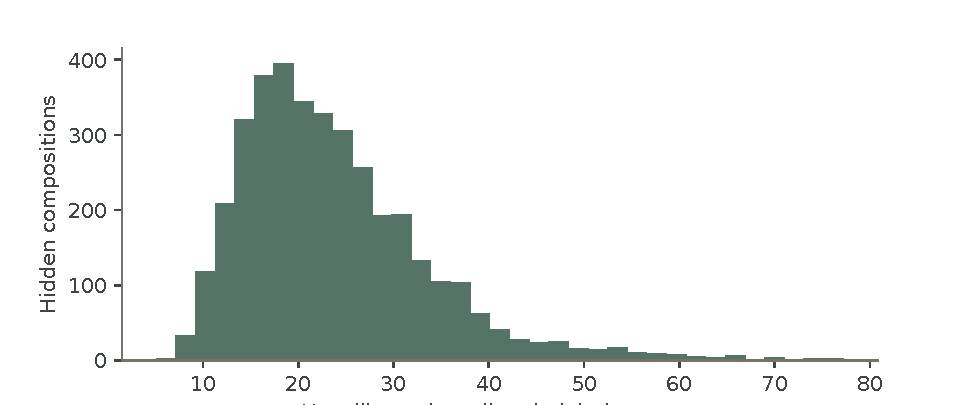
\includegraphics[width=.85\linewidth]{figures/q1_distribution.pdf}\caption{Distribution of Q1 predictions from the 02-only model. Hidden physical labels are unavailable.}\end{figure}
\begin{table}[htbp]\centering\small\caption{First 20 hidden compositions ranked by the Q1 model. All entries are predictions.}\begin{tabular}{rrlr}\toprule Rank & ID & Formula & Score\\\midrule
1 & 5619 & SnZrO2S & 5.0994\\
2 & 18337 & CaNbO2S & 6.6618\\
3 & 5590 & CaTaO2S & 7.2127\\
4 & 2460 & SrNbO2S & 7.2822\\
5 & 3094 & SrNbOFN & 7.3303\\
6 & 18896 & CaNbOFN & 7.4778\\
7 & 11576 & SrTaO2S & 7.4803\\
8 & 6191 & YTiO2S & 7.6029\\
9 & 17664 & BaTaO2S & 7.6791\\
10 & 10869 & CaSnO2S & 7.8212\\
11 & 747 & CaGaO2F & 7.9208\\
12 & 13762 & CdHfO2S & 7.9241\\
13 & 10039 & SrNbO3 & 8.1826\\
14 & 8723 & YTaO2S & 8.2117\\
15 & 12896 & InHfO2S & 8.4206\\
16 & 12933 & BaGaO2F & 8.5014\\
17 & 502 & CaGaO2S & 8.5349\\
18 & 2872 & CaNbO3 & 8.5719\\
19 & 15279 & CaGeO2S & 8.5918\\
20 & 11752 & CaSnO2F & 8.6145\\
\bottomrule\end{tabular}\end{table}


\clearpage
\section{Problems 2 and 3. Exact search on a finite score table}
\subhead{One representative of each metal site}
Let $a_i,b_j\in\{0,1\}$ indicate the selected A and B elements. For Q2 let $C_{ij}=\Vh(i,j,\noo)$. For Q3 store
\begin{equation}
 C_{ij}=\min_{x\in\{\ooo,\noo,\foo\}}\Vh(i,j,x),
 \qquad x^*_{ij}\in\arg\min_x\Vh(i,j,x).
 \label{eq:envelope}
\end{equation}
Taking $\min_{ij}$ in Eq.~\eqref{eq:envelope} visits every eligible triple. Recover $x^*_{ij}$ after choosing the pair, taking the smallest official ID in a tie. A joint one-hot encoding has 156 choices of $(A,X)$ and 52 choices of B. Eliminating X leaves 104 binary variables and a 2,704-cell table. It requires all 8,112 scores in advance. Solving three separate fixed-X problems is another exact decomposition.

For either real cost table, let $D$ denote its min--max normalization. The exactly-one penalty formulation \cite{lucas} is
\begin{equation}
 E(a,b)=\sum_{ij} D_{ij}a_i b_j+
 P\left[\left(\sum_i a_i-1\right)^2+\left(\sum_j b_j-1\right)^2\right].
 \label{eq:qubo}
\end{equation}
Each legal vector activates one cell. Each illegal vector has penalty at least $P$ and nonnegative table cost, so $P>1$ separates it from every legal state before rounding. The encoding represents any predictor evaluated on this finite pool. Requiring the fitted predictor itself to be quadratic would impose an unnecessary restriction.

\subhead{What changes at eight bits?}
Kaiwu converts linear fields to couplings with a reference spin, producing 105 Ising dimensions. Its SPQC documentation specifies signed 8-bit integer couplings \cite{sdk}. We convert Eq.~\eqref{eq:qubo} to Ising, apply the SDK precision adjustment at eight bits, convert back, and compare energies of all 2,704 legal states. We scan $P=1.1,3,10$ using the full Q3 envelope and a version capped at its tenth percentile before normalization. Both tables have the same original minimizer.

\begin{figure}[h]
\centering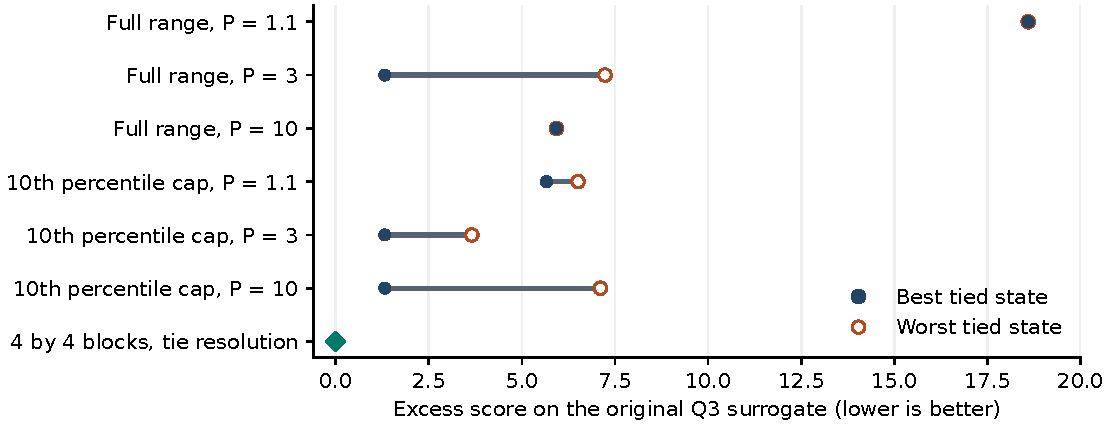
\includegraphics[width=.92\linewidth]{figures/precision.pdf}
\caption{Q3 original-score excess among legal states minimizing each quantized whole-grid energy. A segment spans tied outcomes. Coincident endpoints indicate identical excess. The diamond gives the verified result of the block method.}\label{fig:precision}
\end{figure}

\clearpage
\section{An eight-bit encoding with a checkable minimum}
All six whole-grid configurations in Figure~\ref{fig:precision} lose the minimum of the frozen mixture. For the full range and $P=1.1$, the winning legal pair costs an extra 18.5949 units of $\Vh$. A cap and $P=3$ reduce the best tied excess to 1.3175, still above zero. This audit checks only legal states. We now construct smaller blocks whose entire unconstrained state spaces can be checked.

Sort A and B alphabetically and partition each into thirteen consecutive groups of four. Each of the resulting 169 blocks $T$ covers 16 pairs. Let $M=\max_{ij\in T} C_{ij}$. For nonnegative costs use
\begin{equation}
 q_{ij}=\operatorname{round}(15C_{ij}/M),\quad
 q_{ij}\in\{0,\ldots,15\},\qquad P=16. \label{eq:bins}
\end{equation}
If $M=0$ set the whole block to zero. Use $q$ in Eq.~\eqref{eq:qubo}. A legal state has energy at most 15, whereas every illegal state costs at least 16. Rounding is monotone: the original block minimum is among the rounded minima. Retrieve the complete set of tied minima, read their original costs and keep the least. Comparing the 169 retained original costs recovers the global minimum. This proof depends on retrieving every ground state in a tied block. A sampler returning one arbitrary optimum has a weaker guarantee.

\subhead{Why the coefficients fit}
Write the upper-triangular QUBO with diagonal $-16$, within-group interactions $32$ and cross-group interactions $q_{ij}$, omitting the common constant 32. For eight bits $z$, set $s=2z-1$ and use one reference spin. With Kaiwu's $-s^\mathsf{T}Js$ convention, multiplying the returned symmetric matrix by eight gives integral couplings. Within-group entries are $-32$, cross-group entries are $-q_{ij}$. Each reference coupling is
\begin{equation}
 -\left(2(-16)+3(32)+\sum_{k=1}^4 q_{ik}\right)
 =-\left(64+\sum_{k=1}^4 q_{ik}\right),
\end{equation}
using the corresponding column sum on the B side. Its magnitude is at most 124. This is an a priori 8-bit bound for every block, independent of the absolute units of $\Vh$.

Kaiwu's \texttt{BruteForceOptimizer} solves the resulting nine-spin instances on the local CPU. We fix the gauge by multiplying every spin by the reference spin and deduplicate binary states. An independent pass checks all $2^8=256$ assignments in each block, including infeasible assignments. It verifies the affine energy relation, counts ground states, and compares every decoded optimum with the integer-cost table. Across both pools all 338 calls return complete sets of feasible ground states. Every retained block winner also matches the minimum of its original floating-point block.

\clearpage
\section{Selected compositions and computational cost}
\begin{table}[h]
\caption{Answers and membership checks. The two full pools are solved by Kaiwu. Direct scans of the two blind subsets give the restricted-pool comparison.}\label{tab:answers}
\centering\small\begin{tabular}{llrllrr}
\toprule Task & Pool (size) & ID & $(A,B,X)$ & Formula & $\Vh$ & Public $V$\\\midrule
Q2 & 07 (2,704)&13153& La, Ti, NO2 & LaTiO$_2$N & 6.924382 & hidden\\
Q3 & 08 (8,112)&8760& Sn, Ti, O3 & SnTiO$_3$ & 3.268113 & 0.001419\\\midrule
Q2 & 11 (529)&13153& La, Ti, NO2 & LaTiO$_2$N & 6.924382 & hidden\\
Q3 & 12 (1,587)&13153& La, Ti, NO2 & LaTiO$_2$N & 6.924382 & hidden\\\bottomrule
\end{tabular}
\end{table}
The winners in Table~\ref{tab:answers} use the same refitted model. The ordered triplets explain why the file's NO2 family is written as O$_2$N in the supplied formula. For Q2 and Q3, respectively, runner-up scores are 7.256664 and 3.904881. Enumeration gaps for the chosen records are zero. Their winning-block Ising energies under $-s^\mathsf{T}Js$ are $-702$ and $-724$. Constants and scales vary by block, so comparing those two energies would have no physical meaning. $\mathrm{SnTiO_3}$ belongs to file 02; its public value is an in-training observation after refitting. For a new DFT calculation in the blind pool, both objectives nominate $\mathrm{LaTiO_2N}$.

\begin{table}[h]
\caption{Wall-clock measurements on an AMD Ryzen 9 8945HX CPU. Fitting the three-component model is shared across both optimization problems.}\label{tab:cost}
\centering\small\begin{tabular}{lrr}
\toprule Stage & Q2 & Q3\\\midrule
Descriptors, shared (s) & \multicolumn{2}{c}{\DescFull}\\
Refit on 15,225 rows, shared (s) & \multicolumn{2}{c}{\FitFull}\\
Score 8,112 rows, shared (s) & \multicolumn{2}{c}{\ScoreFull}\\
Subset, index and reduce pool (s) & \PoolTwo & \PoolThree\\
Construct and convert 169 blocks (s) & \EncodeTwo & \EncodeThree\\
169 Kaiwu CPU solves (s) & \SolveTwo & \SolveThree\\
Decode, resolve ties, verify (s) & \CheckTwo & \CheckThree\\
Direct array minimum, median ($\mu$s) & \ScanTwo & \ScanThree\\
Blocks with ties / 169 & \TiedTwo & \TiedThree\\
Original costs compared within tied or unique minima & \FinalistsTwo & \FinalistsThree\\
Observed integer coupling range & $[\CoeffLowTwo,0]$ & $[\CoeffLowThree,0]$\\\bottomrule
\end{tabular}
\end{table}
The direct scan uses the same in-memory predictions and times 1,001 repetitions of one array minimum. The larger QUBO times include the checks itemized above; disk I/O and manuscript generation lie outside these timings. For Q1 alone, descriptors, training and scoring the hidden set took \DescOne, \FitOne\ and \ScoreOne\ seconds. These are local wall times under the observed machine load. Device programming, queueing, sampling, energy consumption and hardware success rates remain unmeasured.

\clearpage
\section{Interpretation and limits}
Two kinds of error matter to a one-composition decision. For any returned candidate $u$ and a true minimizer $u^*$ in the same pool, adding and subtracting predicted scores yields
\begin{equation}
 V(u)-V(u^*)\ \leq\
 2\max_{z}|V(z)-\Vh(z)|+
 \underbrace{\Vh(u)-\min_z\Vh(z)}_{\text{optimization gap}} .
 \label{eq:regret}
\end{equation}
The maximum is taken over that pool. The second term is exactly zero for our full-pool results. The first term cannot be estimated uniformly on hidden compositions from a mean validation error. For example, even selecting the exact minimum of the primary surrogate on Q3 validation incurs physical regret 11.45225. Two models that agree on average can still disagree where the minimum lies.

The metallic lower bound exploits an empirical identity in this particular dataset and can transfer only where the energy conventions remain valid. A single material outside the assumed branch may give a confident wrong choice. In the unseen-pair folds the mixture finds 23 of 50 three-family near-targets at 50 checks per fold, compared with 14 for direct regression. Their median single-choice regrets are 13.521 and 11.569, respectively. These measurements support shortlist enrichment more strongly than a one-shot prediction. A physical calculation for the blind winner would provide information unavailable from any additional optimization of the frozen scores.

The eight-bit construction controls a different risk. Small, exactly solved blocks allow the original-score minimum to survive ties, while increasing classical work. A large hardware instance has programming and readout costs and may miss tied ground states. Benchmarking a device would require observed success probabilities and end-to-end timings on comparable inputs \cite{speed}. In the present search, every composition is scored before optimization, and a direct scan already attains the same minimum in microseconds. The experiment establishes finite-precision correctness on the local Kaiwu backend. The performance and physical outcome of an SPQC run remain open.

For the requested full pools the single choices are therefore $\mathrm{LaTiO_2N}$ for Q2 and $\mathrm{SnTiO_3}$ for Q3. If the next action is to assay an unlabeled composition, the common blind-pool choice is $\mathrm{LaTiO_2N}$. Its predicted score of 6.924382 leaves its physical status unresolved.


\clearpage
\begin{thebibliography}{11}
\bibitem{castelli} Castelli I. E., Landis D. D., Thygesen K. S., Dahl S., Chorkendorff I., Jaramillo T. F., Jacobsen K. W., New cubic perovskites for one- and two-photon water splitting using the computational materials repository [J], Energy \& Environmental Science, 2012, 5, 9034--9043. \url{https://doi.org/10.1039/C2EE22341D}.
\bibitem{contest} APMCM Organizing Committee, Problem D: Application of Special Purpose Quantum Computer to Rare-Target Search in Perovskite Candidate Materials, official problem statement and accompanying dataset notes, 2026.
\bibitem{aflow} AFLOW Encyclopedia of Crystallographic Prototypes, Cubic Perovskite (CaTiO$_3$) Structure, \url{https://aflow.org/p/AB3C_cP5_221_a_c_b-001/}, accessed 2026-11-26.
\bibitem{kuisma} Kuisma M., Ojanen J., Enkovaara J., Rantala T. T., Kohn--Sham potential with discontinuity for band gap materials [J], Physical Review B, 2010, 82, 115106. \url{https://doi.org/10.1103/PhysRevB.82.115106}.
\bibitem{ward} Ward L., Agrawal A., Choudhary A., Wolverton C., A general-purpose machine learning framework for predicting properties of inorganic materials [J], npj Computational Materials, 2016, 2, 16028. \url{https://doi.org/10.1038/npjcompumats.2016.28}.
\bibitem{ong} Ong S. P., Richards W. D., Jain A., Hautier G., Kocher M., Cholia S., Gunter D., Chevrier V. L., Persson K. A., Ceder G., Python Materials Genomics (pymatgen): A robust, open-source python library for materials analysis [J], Computational Materials Science, 2013, 68, 314--319. \url{https://doi.org/10.1016/j.commatsci.2012.10.028}.
\bibitem{catboost} Prokhorenkova L., Gusev G., Vorobev A., Dorogush A. V., Gulin A., CatBoost: unbiased boosting with categorical features [C], Advances in Neural Information Processing Systems, 2018, 31.
\bibitem{note1} Shumo Jiayouzhan, AI-assisted ideas for 2026 APMCM Problem D [translated title], Xiaohongshu, \url{https://xhslink.cn/o/5LxZKskY5UK}, accessed 2026-11-26.
\bibitem{note2} Shuxue Jianmo Laoge, A solution approach to 2026 APMCM Problem D [translated title], Xiaohongshu, \url{https://xhslink.cn/o/4SqQmBiyKO6}, accessed 2026-11-26.
\bibitem{lucas} Lucas A., Ising formulations of many NP problems [J], Frontiers in Physics, 2014, 2, 5. \url{https://doi.org/10.3389/fphy.2014.00005}.
\bibitem{sdk} QBoson, Ising matrix precision adaptation, Kaiwu SDK documentation, \url{https://kaiwu-sdk-docs.qboson.com/zh/latest/source/advanced/precision.html}, accessed 2026-11-26.
\bibitem{speed} R{\o}nnow T. F., Wang Z., Job J., Boixo S., Isakov S. V., Wecker D., Martinis J. M., Lidar D. A., Troyer M., Defining and detecting quantum speedup [J], Science, 2014, 345, 420--424. \url{https://doi.org/10.1126/science.1252319}.
\end{thebibliography}


\clearpage
\section*{Appendix. Reproduction and complete source listings}
\phantomsection
\addcontentsline{toc}{section}{Appendix. Reproduction and complete source listings}
Python 3.12.14, CatBoost 1.2.10, pymatgen 2025.10.7, NumPy 2.5.5, pandas 2.2.3, SciPy 1.18.1, scikit-learn 1.9.1 and Kaiwu SDK 1.4.4 were used on Windows 11. Figures use the ideal cubic prototype, public physical properties, saved predictions and solver tables. Matplotlib 3.10.3 produced the vector figures and XeLaTeX typeset the manuscript with the supplied APMCM class.

Place the original files in \texttt{problem\_d/date}. Run the data audit, the validation and stress comparisons for seeds 26 and 42, the physical-property comparison, the seed-26 encoding and precision audit, then the paper scripts. Running \texttt{screen.py scores} produces the hidden Q1 predictions and the refit Q2/Q3 score table. Running \texttt{screen.py development} produces the five-fold results. Use \texttt{solve.py} for both full-pool searches, then \texttt{figures.py}, \texttt{material\_figures.py}, \texttt{perovskite\_plates.py} and \texttt{tables.py} for the manuscript. The companion README gives the arguments and file names for each call.

The score ledger records SHA-256 digests for the two exported tables. The block ledger contains the selected ID, tie count, integer-energy minimum, scaled Ising energy, observed coupling range and timing for each call. Both final-pool selections can be reconstructed from the tables alone.

\lstset{language=Python,basicstyle=\fontsize{8.5}{10}\selectfont\ttfamily,
  columns=fullflexible,keepspaces=true,breaklines=true,breakatwhitespace=false,
  frame=none,backgroundcolor=\color{white},rulecolor=\color{white},
  keywordstyle=\color{black},stringstyle=\color{black},commentstyle=\color{black!65},
  aboveskip=2pt,belowskip=4pt,showstringspaces=false}
\newcommand{\program}[2]{\clearpage\subhead{#1}\lstinputlisting{#2}}
\program{A1. Surrogate features and model components}{../exploration/compare_surrogates.py}
\program{A2. Source checks and label reconstruction}{../exploration/audit_data.py}
\program{A3. Withheld near-target and encoding experiments}{../exploration/test_innovation_ideas.py}
\program{A4. Physical-property-first prediction}{../exploration/compare_physical_properties.py}
\program{A5. Whole-grid SDK precision audit}{../exploration/audit_sdk_precision.py}
\program{A6. Frozen predictions and grouped folds}{screen.py}
\program{A7. Integer QUBO construction, exact solution and checks}{solve.py}
\program{A8. Manuscript figures}{figures.py}
\program{A9. Measured values for the manuscript tables}{tables.py}
\program{A10. Crystal geometry and screening diagnostics}{material_figures.py}
\program{A11. Perovskite structure, band edges and anion compositions}{perovskite_plates.py}

\end{document}

